\section{实验目的}

\begin{enumerate}
    \item 熟悉加减法器的使用方法;
    \item 掌握 ALU 的组成原理。
\end{enumerate}

\section{实验内容}

\begin{enumerate}
    \item 测试加减法器的功能;
    \item 设计具有加,减,按位与,按位取反四种功能的 ALU。
\end{enumerate}

\section{实验原理及设计}

测试加减法器的过程略。

\subsection{功能约定}

约定 ALU 的各个端口功能见表 \ref{table:2-func}。

\begin{table}[h]
    \centering
    \caption{ALU 端口功能表}
    \label{table:2-func}
    \begin{tabular}{|c|c|c|}
        \hline
        端口名称 & 端口宽度 & 端口说明 \\ \hline
        \verb|Op| & 2 & ALU 的功能选择端口,具体功能见表 \ref{table:2-func_code} \\ \hline
        \verb|A| & 8 & 第一操作数 A,有符号整数 \\ \hline
        \verb|B| & 8 & 第二操作数 B,有符号整数 \\ \hline
        \verb|F| & 8 & 运算结果,有符号整数 \\ \hline
        \verb|OF| & 1 & 溢出指示符号位 \\ \hline
        \verb|CF| & 1 & 进借位指示符号位 \\ \hline
        \verb|ZF| & 1 & 零用指示符号位 \\ \hline
        \verb|SF| & 1 & 运算结果符号位 \\ \hline
    \end{tabular}
\end{table}

\begin{table}[h]
    \centering
    \caption{ALU 功能编码表}
    \label{table:2-func_code}
    \begin{tabular}{|c|c|c|}
        \hline
        编码 & 功能名称 & 备注 \\ \hline
        \verb|00| & 加法 & 有符号 \\ \hline
        \verb|01| & 减法 & 有符号 \\ \hline
        \verb|10| & 按位与 & 除 \verb|ZF| 以外的符号位行为未定义 \\ \hline
        \verb|11| & 按位取反 & 仅 A 参与运算,除 \verb|ZF| 以外的符号位行为未定义 \\ \hline
    \end{tabular}
\end{table}

\subsection{电路设计}

加减法直接使用 ALU 进行计算。另外,按位与和按位取反需要另外的逻辑门实现,最后输出时将输出连接到数据选择器,
让数据选择器选择正确的输出即可。

然后考虑如何设计各个指示信号:

\begin{itemize}
    \item \verb|OF| 信号直接使用加减法器的输出即可。
    \item \verb|CF| 是针对无符号运算而言的。按照进借位判定方法,可以采用\verb|Cout XOR ~Op| 来实现。
    \item \verb|SF| 直接输出运算结果的最高位即 \verb|F[7]| 即可。
    \item \verb|ZF| 输出运算结果的各位或的结果取反即可。
\end{itemize}

设计电路图如图 \ref{figure:2-design} 所示:

\begin{figure}[h]
    \centering
    \caption{ALU 设计图}
    \label{figure:2-design}
    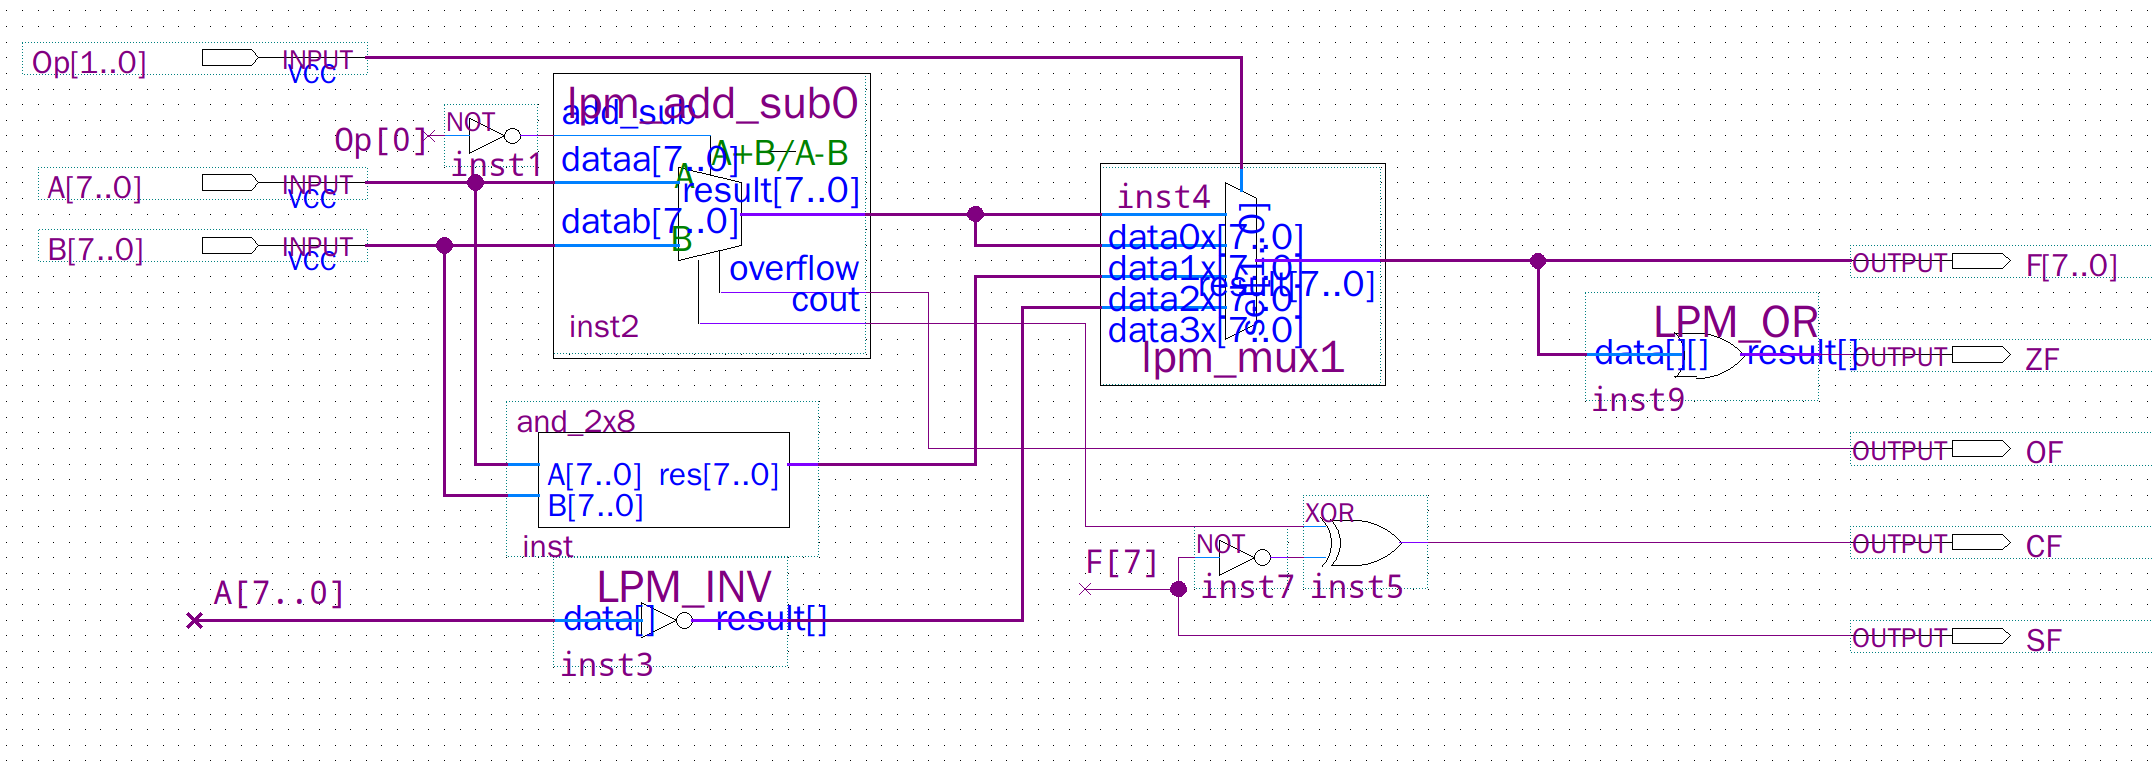
\includegraphics[scale=0.2]{pics/2-design.png}
\end{figure}

其中:
\begin{itemize}
    \item \verb|LPM_OR| 的各参数取值如下:
    \begin{itemize}
        \item \verb|LPM_WIDTH|:1
        \item \verb|LPM_SIZE|:8
    \end{itemize}
    \item \verb|and_2x8| 为自定义的元件,实现了将 2 个 8 位数据按位或的功能,定义文件为\verb|and_2x8.v|,
    具体代码见源代码 listing \ref{listing:and_2x8}。
\end{itemize}

\begin{listing}[h]
    \caption{\texttt{and\_2x8} 代码定义}
    \label{listing:and_2x8}
    \begin{minted}[linenos=true,autogobble,bgcolor=mintbg]{verilog}
module and_2x8(
    input[7:0] A,
    input[7:0] B,
    output[7:0] res
);
    assign res[7:0] = {
        A[7] & B[7],
        A[6] & B[7],
        A[5] & B[5],
        A[4] & B[4],
        A[3] & B[3],
        A[2] & B[2],
        A[1] & B[1],
        A[0] & B[0]
    };
endmodule
    \end{minted}
\end{listing}

\section{实验结果}

实验使用的输入波形与输出波形如图 \ref{figure:2-result} 所示。

\begin{figure}
    \centering
    \caption{ALU 功能验证结果}
    \label{figure:2-result}
    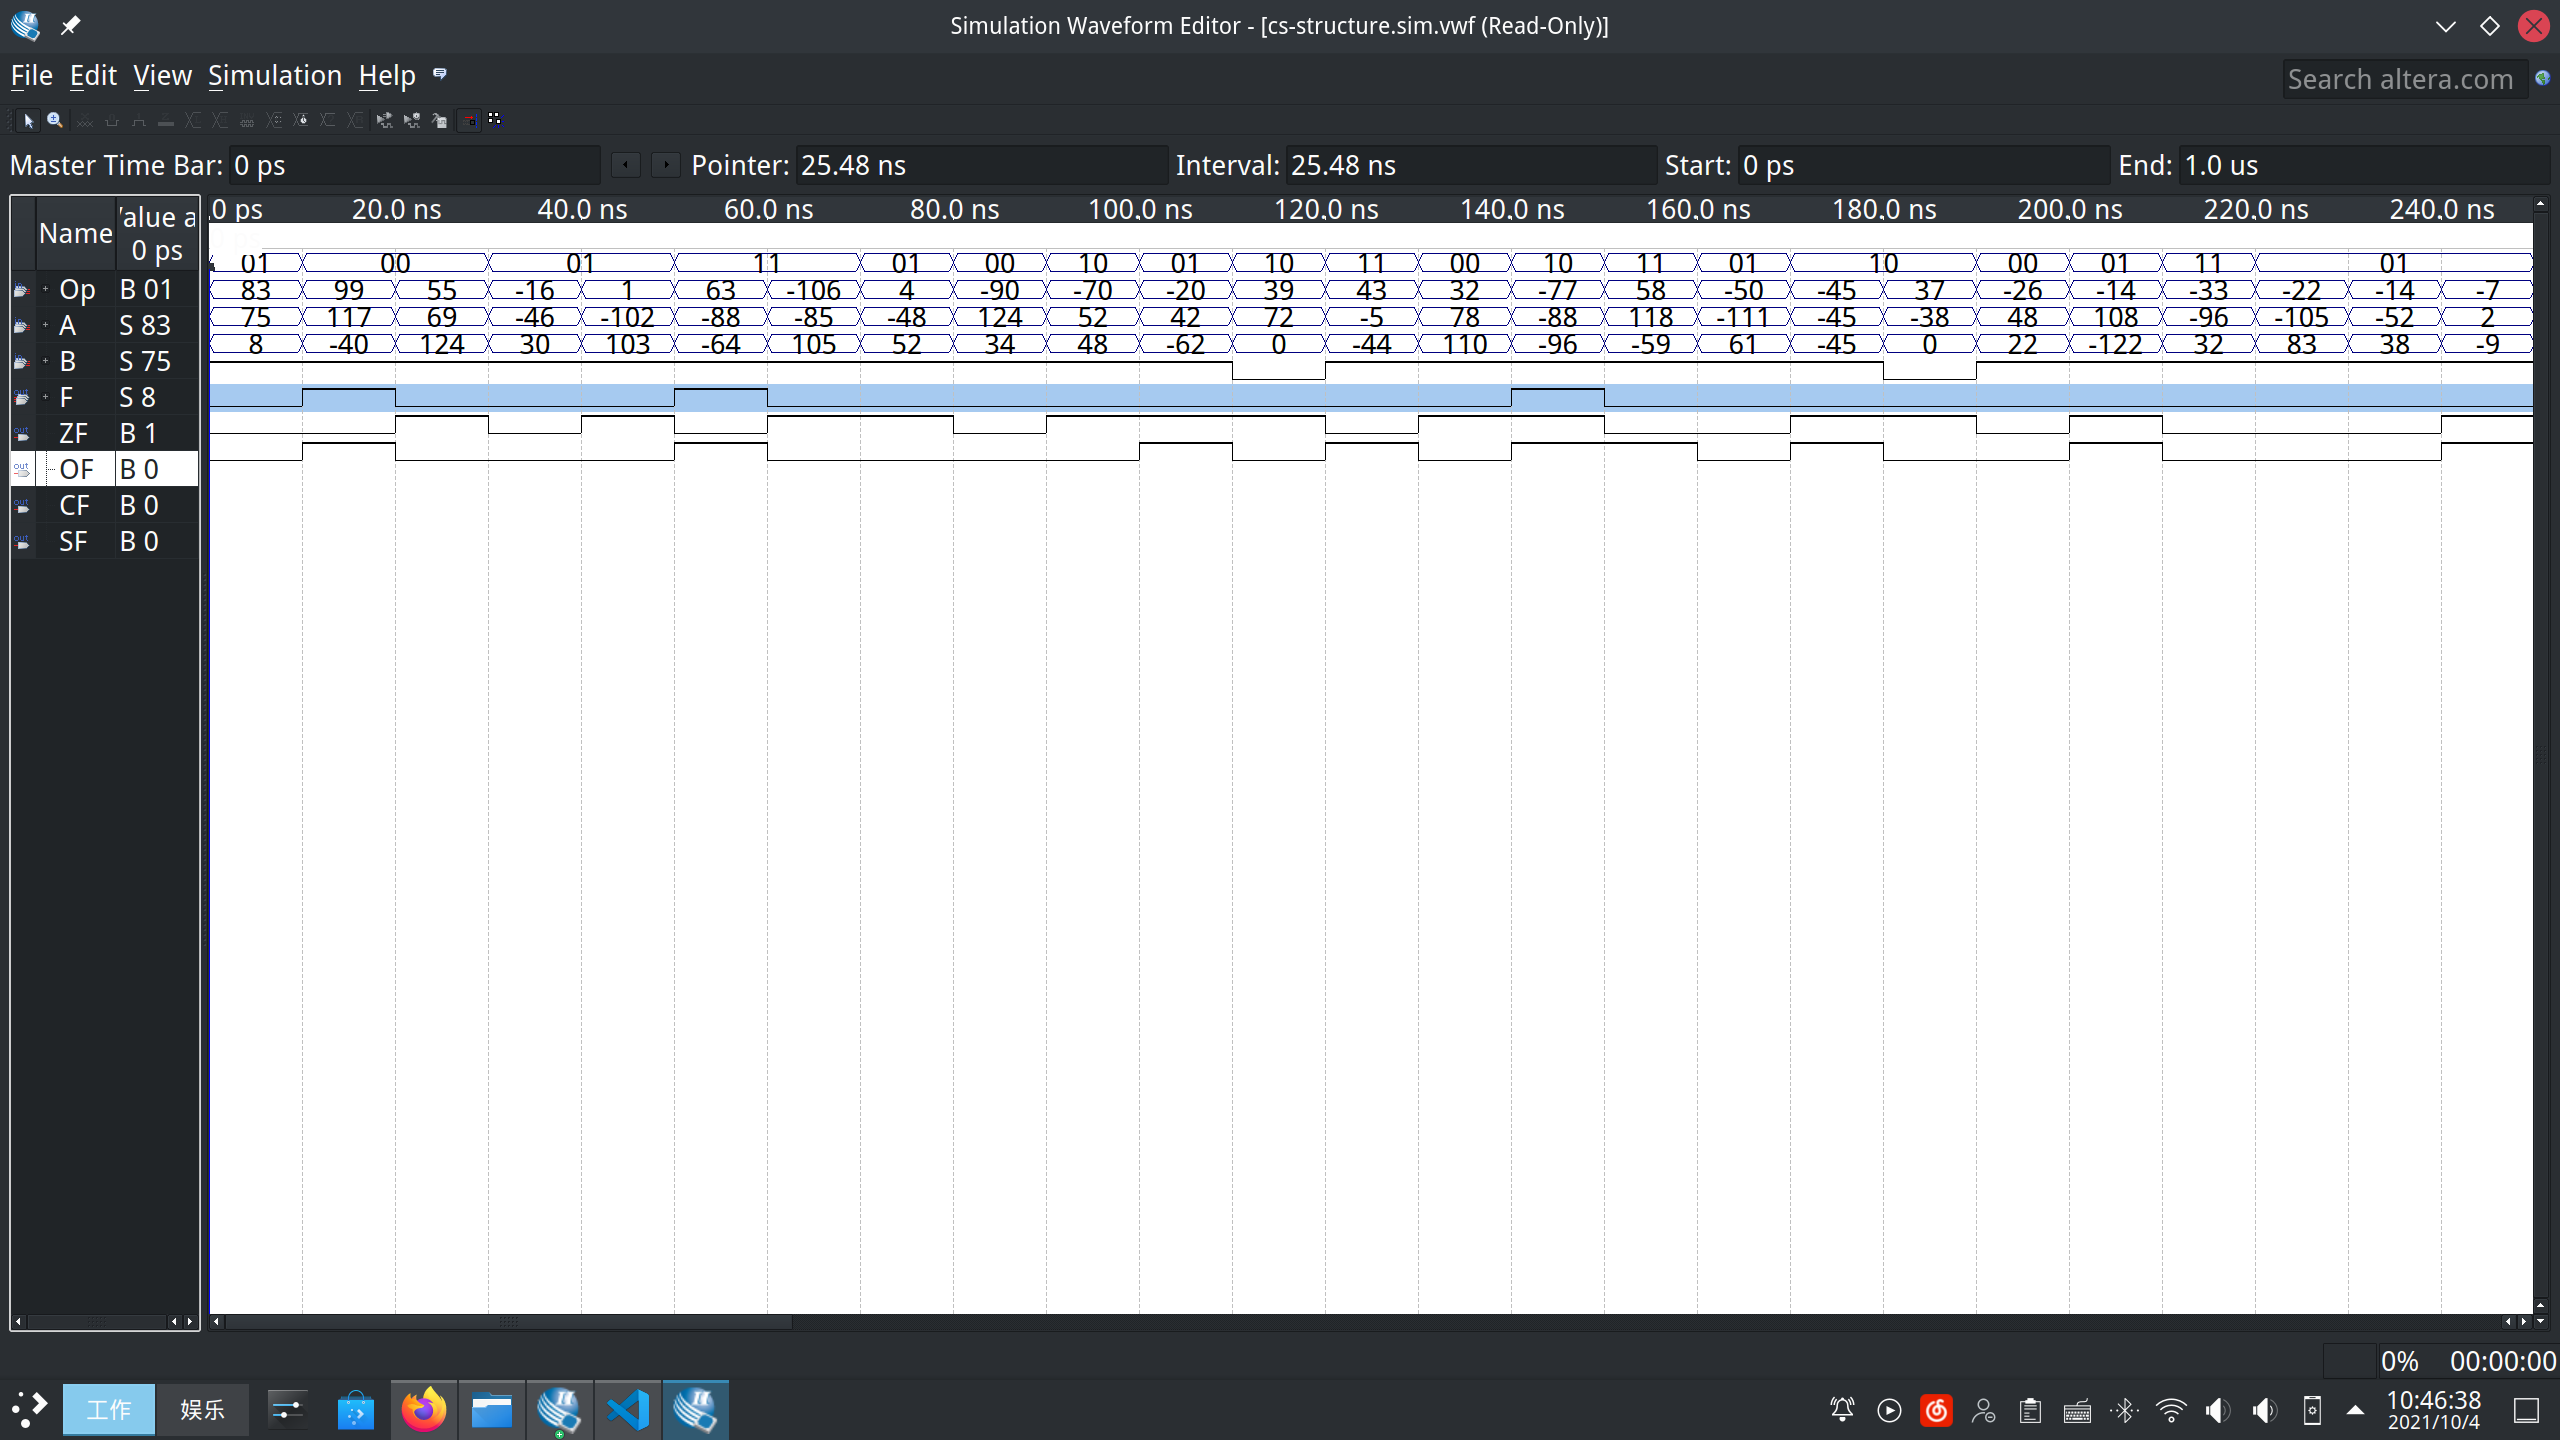
\includegraphics[scale=0.2]{pics/2-result.png}
\end{figure}

结果表明,ALU 的功能正常。

\section{源文件列表}

见表 \ref{table:2-files}。

\begin{table}[h]
    \centering
    \caption{ALU 设计实验文件列表}
    \label{table:2-files}
    \begin{tabular}{|c|c|}
        \hline
        文件名称 & 说明 \\ \hline
        \verb|test_alu.bdf| & ALU 设计图文件 \\ \hline
        \verb|test_alu.vwf| & ALU 测试波形文件 \\ \hline
        \verb|and_2x8.v| & 元件 \verb|and_2x8| 的代码实现 \\ \hline
        \verb|test_add_sub.bdf| & 测试加法器功能的设计图文件 \\ \hline
        \verb|test_add_sub.vwf| & 测试加法器功能的波形文件 \\ \hline
        \verb|lpm_mux1.qip| & 四选一选择器 \verb|lpm_mux1| 的实例文件 \\ \hline
    \end{tabular}
\end{table}